\documentclass{article}

% ************* Preamble *************************** 
% Language setting
% Replace `english' with e.g. `spanish' to change the document language
\usepackage[english]{babel}

% Set page size and margins
% Replace `letterpaper' with`a4paper' for UK/EU standard size
% \usepackage[a4paper,top=2cm,bottom=2cm,left=3cm,right=3cm,marginparwidth=1.75cm]{geometry}
\usepackage[a4paper]{geometry}

% Useful packages
\usepackage{amsmath}
\usepackage{graphicx}
\graphicspath{{../figures/}}
% \usepackage[colorlinks=true, allcolors=blue]{hyperref}
\usepackage{hyperref}
\usepackage{blindtext} % to generate 2 pages of text
\usepackage{threeparttable}
\usepackage{booktabs} % nicer tables w/ mid, top, bottom rules
\usepackage{dcolumn} % should align decimals in tables
\newcolumntype{d}[1]{D{.}{.}{#1}} % command for dcolumn, use d{2} instead of l,
% or c in tabular column specifier

% Biblatex (options taken from Igors Github, is it equal to JoF style?)
\usepackage[
    backend=biber,
    style=bwl-FU,
    url=false,
    doi=false,
    eprint=false
]{biblatex}
\addbibresource{references.bib}

% Title
\title{DTFF Final Project Paper\thanks{Thanks to Alice, Bob, Charlie and Dan for their helpful support.}}
\author{Egemen Erdogdu\thanks{Egemen Erdogdu, University of Zurich, Rämistrasse 71, 8006 Zürich} \\ University of Zurich \and Jonas Schmidiger\thanks{Jonas Schmidiger, University of Zurich, Rämistrasse 71, 8006 Zürich} \\ University of Zurich \and Mathias Ruoss\thanks{Mathias Ruoss, University of Zurich, Rämistrasse 71, 8006 Zürich}\\ University of Zurich}
\date{\today}


% *************** Document ***********************
\begin{document}
\maketitle
% \thispagestyle{empty} % to surpress page numbering in title page
\begin{abstract}
    This abstract is a groundbreaking summary.
    \blindtext
\end{abstract}



% table of contents
\newpage
\tableofcontents
\newpage

\section{Introduction}
\blindtext[2]


% \blinddocument

% Citations
This is a first citation (\cite{Kozlowski2020}). This is a second citation (\cite{Gormsen2020}).

\section{Background}
\blindtext[2]

\section{Dataset}
\blindtext[2]
% Table
% \begin{table}
%     \centering
%     \begin{threeparttable}
%         \caption{This is our first table.} %Title to be above table
%         \begin{tabular}[t]{lcc}
%         &Column1&Columm2\\
%         \hline
%         John Smith&10&12\\
%         Jane Doe&15&9\\
%         Mary Johnson&10&18\\
%         \end{tabular}
%         \begin{tablenotes}
%             \item{Note:} Some random table note. % Note of table
%         \end{tablenotes}
%     \end{threeparttable}
%     \label{table:1}
% \end{table}

\begin{table}
    \centering
    \caption{Summary Statistics}
    \begin{tabular}{@{}ld{3}d{3}d{3}d{3}d{3}d{3}@{}}
    \toprule
    \multicolumn{1}{l}{Stock}       & \multicolumn{1}{c}{FB} & \multicolumn{1}{c}{AMZN} & \multicolumn{1}{c}{AAPL} & \multicolumn{1}{c}{NFLX} & \multicolumn{1}{c}{GOOGL} &  \\ \midrule
    Panel A: Descriptive statistics &        &        &        &        &        &  \\ \midrule
    Mean                            & 0.083  & 0.065  & 0.112  & 0.051  & 0.091  &  \\
    Variance                        & 0.041  & 0.030  & 0.044  & 0.061  & 0.037  &  \\
    Median                          & 0.064  & 0.058  & 0.091  & 0.043  & 0.102  &  \\
    Maximum                         & 0.053  & 0.064  & 0.078  & 0.043  & 0.062  &  \\
    Minimum                         & -0.211 & -0.181 & -0.195 & -0.203 & -0.081 &  \\
    Jarque Bera                     & 95.35   & 81.54   & 49.27   & 40.58   & 0.58   &  \\ \bottomrule
    \end{tabular}
    \begin{tablenotes}
        \item{Note:} Some random table note. % Note of table
    \end{tablenotes}
    \label{tab:summary_stat}
\end{table}


\section{Methods}
\blindtext[2]

\section{Results}
\blindtext[2]
% Graphic
% \begin{figure}[t]
%     % \centering
%     \caption{This is our first figure, taken from Igor's Github repo.}
%     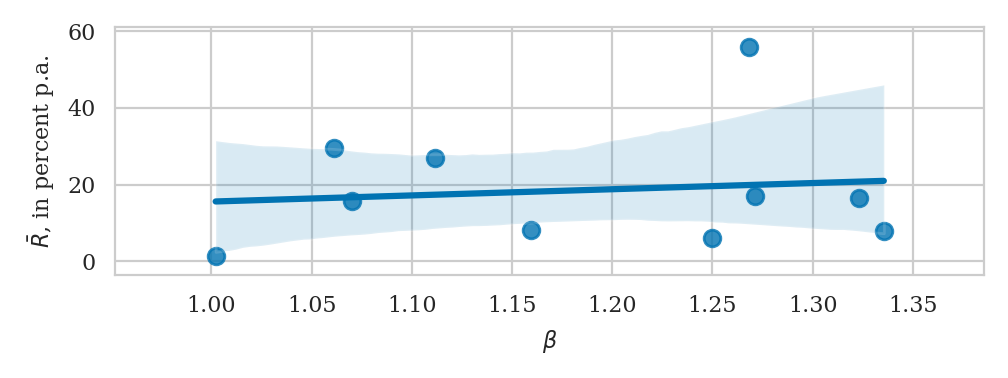
\includegraphics[width=\textwidth]{beta-vs-mu}
%     Note: Some random figure note.
%     \label{fig:1}
% \end{figure}

\begin{figure}
    \centering
    \caption{Cumulative Returns of FAANG stocks}    
    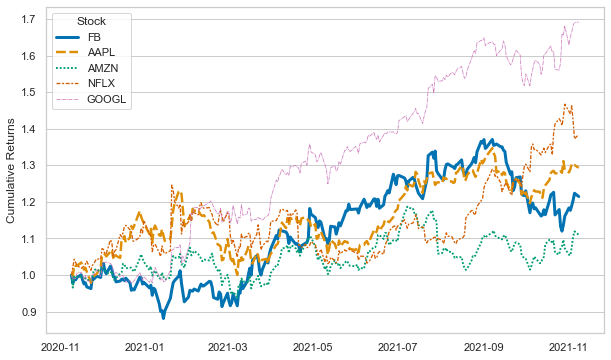
\includegraphics[width=\linewidth]{lineplot_paper}
    \label{fig:cum_ret_faang}
  \end{figure}        

\section{Conclusion}
\blindtext[2]

 
% Clearpage better than \newpage (prints all figures and tables before adding bibliography on a new page)
\clearpage
\printbibliography

\end{document}
